\chapter{Evaluation}

In our project, the dataset we used was crawled from 
\url{http://www.avsforum.com/f/}. The forum deals mainly with Audio-Visual 
equipment, with discussions about technical details, offers and people showing 
off their DIY projects.

The forum was chosen from the list which \outcite{Yang2009} provided in their 
paper. The forum users use mainly proper English, which made removing stopwords 
and stemming simpler.

We crawled 4,158 threads, with a total of 1,002,225 posts. A distribution of how 
the length of threads are distributed can be seen in Figure \ref{fig:len_dist}.  
The distribution of the time differences are shown in Figure \ref{fig:dt_dist}.  
In both the figures, the right-hand-side cutoff was set at 1,000 due to the 
negligible number of items to the right of the cutoff.


\putgraphic{diagrams/len_dist.png}{Distribution of thread 
length}{len_dist}{0.75}
\putgraphic{diagrams/time_dist.png}{Distribution of $\dt$}{dt_dist}{0.75}

We have also found that the time of the day the day of the week matters when 
dealing with threads. An example of such a thread can be seen in Figure 
\ref{fig:hr_freq} and Figure \ref{fig:week_freq}, where we see that activity 
peaks at 2 PM, dropping slightly during (an assumed) lunch period, and then 
peaks again during the early evening and at 9 PM.  Activity drops to its lowest 
at 3 AM. The weekly graph also shows a pattern, showing lower posting 
frequencies during the weekends, and its highest peak on Thursdays.
\begin{figure}
\begin{center}
\begin{subfigure}[b]{0.45\textwidth}
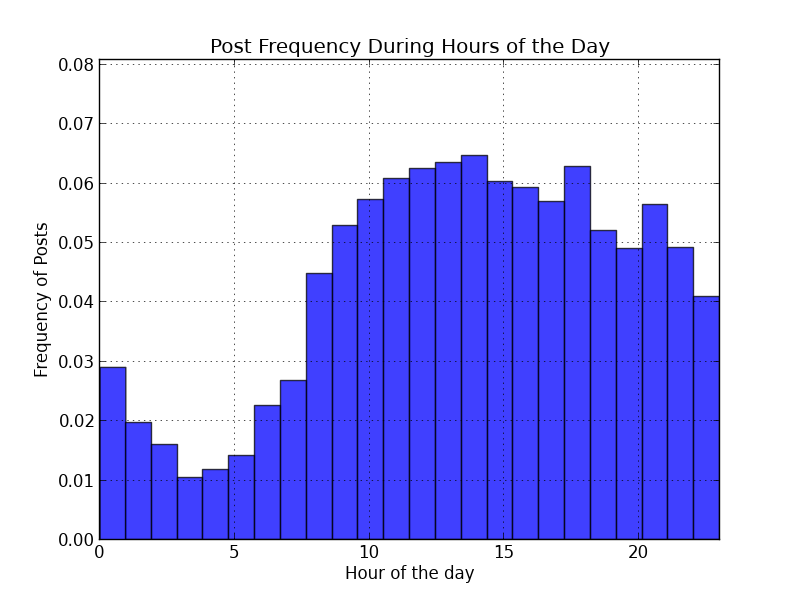
\includegraphics[width=\textwidth]{diagrams/hoursofday.png}
\caption{The hourly post frequency.}
\label{fig:hr_freq}
	\end{subfigure}
	\begin{subfigure}[b]{0.45\textwidth}
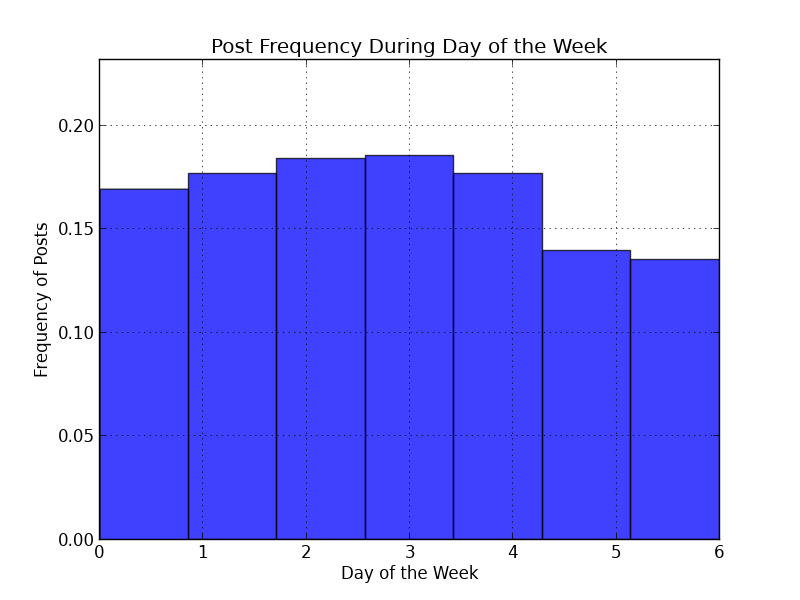
\includegraphics[width=\textwidth]{diagrams/daysofweek.png}
\caption{The daily post frequency.}
\label{fig:week_freq}
	\end{subfigure}
\end{center}
\end{figure}




\section{Experiment setup}
The first 75\% of the thread was used as training data, while the remaining 25\% 
was used as test data. This setup is used in both the tuning of parameters and 
for the full evaluation of the entire dataset.
%\begin{figure}
%	\input{diagrams/exp_setup}
%	\caption{Our experiment setup}
%	\label{fig:exp_setup}
%\end{figure}

\subsection{Parameter Tuning}
Before we begin performing experiments on the full dataset, we first tuned the 
machine learning algorithms using a sample of the forum threads. In the 
following experiments, the threads chosen from our extracted dataset are those 
with a 100 to 200 posts. This amounted to 97 threads. In each of these 
experiments, we run the algorithm with different parameters, and use the optimal 
one in our final evaluation. 

\subsubsection{Vocabulary size}
Before we begin tuning the other parameters, we start with limiting the size of 
the feature vector when using the content information. This is important as 
having an excessively large feature vector due to a large vocabulary size leads 
to complications due to limited memory size. We restrict our search for a good 
size of vocabulary from $10 \leq K \leq 60$, with increments of 10.  The results 
are shown in Table \ref{table:vocab_exp}. While $K=60$ gives us the best 
$T$-score, we select $K=50$ as this gives us the best $\Prerror$ score.  
\begin{table}
	\footnotesize
\begin{center}
	\begin{tabular}{|l|c|c|c|c|c|c|c|c|}
	\hline
& $T$-score			   &	Visit/Post & 	$\prerror$\\
	\hline
	\input{tables/vocab_exp}
	\hline
	\end{tabular}
\end{center}
	\caption{Experiment results: Varying vocabulary size}
	\label{table:vocab_exp}
\end{table}



\subsubsection{Window size}
Using a combination of feature sets, we experiment with different window sizes, 
$w = 1, 5, 10, 15$.

Performing the experiment using only the $\dt$ values within the window, we 
obtain the results found in Table \ref{tbl:par_tune_dt}. The results show that 
$w=15$ provide the best $T$-score. We must however, keep in mind that its 
Visit/Post ratio is the highest, but also has a higher standard error.

\begin{table}
	\footnotesize
\begin{center}
\begin{tabular}{| l | c | c | c |}
\hline
& $T$-score			   &	Visit/Post & 	$\prerror$\\
\hline
	\input{tables/dt_vec_features}
\hline
\end{tabular}
\end{center}
\caption{Results for tuning parameters using only 
$\dtvec$}\label{tbl:par_tune_dt}
\end{table}

Using only the content, we perform the same experiment again. This gives us the 
results in Table \ref{tbl:par_tune_content}. The best $T$-score here does not do 
as well as that in the previous experiment. However, it is interesting to note 
that, again, $w=15$ results in the best $T$-score.

\begin{table}
	\footnotesize
\begin{center}
\begin{tabular}{| l | c | c | c |}
\hline
& $T$-score			   &	Visit/Post & 	$\prerror$\\
\hline
	\input{tables/word_vec_features}
\hline
\end{tabular}
\end{center}
\caption{Results for tuning parameters using only 
$\vocab$}\label{tbl:par_tune_content}
\end{table}

For our final experiment for tuning the window size, we combine the various 
feature sets together. We also include the time-context in this experiment, and 
we arrive at the results found in Table \ref{tbl:par_tune_comb}. Again, $w=15$ 
has the best $T$-score, but only with a slight improvement over our first 
experiment.

In any case, this suggests that $w=15$ may be the best window size. In the 
following experiments, this will be our $w$ value.

\begin{table}
	\footnotesize
\begin{center}
\begin{tabular}{| l | c | c | c |}
\hline
& $T$-score			   &	Visit/Post & 	$\prerror$\\
\hline
\input{tables/comb_vec_features}
\hline
\end{tabular}
\end{center}
\caption{Results for tuning parameters using $\dtvec+ \vocab+ 
\ctxvec$}\label{tbl:par_tune_comb}
\end{table}


\subsubsection{Decay factor}
In our discounted sum method, we have to tune the $\alpha$ parameter. We search 
through 0.1 to 0.9 (inclusive) with increments of 0.1 to find the best possible 
value for $\alpha$.  We used the combined set of features for this experiment.
The results are shown in Table \ref{tbl:par_tune_decay}.
\begin{table}
	\footnotesize
\begin{center}
\begin{tabular}{| l | c | c | c |}
\hline
& $T$-score			   &	Visit/Post & 	$\prerror$\\
\hline
	\input{tables/alpha_decay}
\hline
\end{tabular}
\end{center}
\caption{Results for tuning $\alpha$ for the \texttt{DEC} 
method}\label{tbl:par_tune_decay}
\end{table}

$\alpha=0.9$ performs the best, but its improvement over the rest of the values 
for $\alpha$ are not by much. Also, note that the $T$-scores do not defer much 
from the previous experiment, although there is a slight improvement.

\subsubsection{Learning rate for Stochastic Gradient Descent}

Because of the scaling factors applied to the sigmoid function, a small change 
in the exponent of $e$ results in huge fluctuations. As such, we need to find a 
small enough learning rate such that the predicted values do not end up at only 
the extremes ($\lambda$ or $\Lambda$), but large enough such that the model is 
adaptive enough to ``react" to changes.

\begin{table}
	\footnotesize
\begin{center}
\begin{tabular}{| l | c | c | c |}
\hline
& $T$-score			   &	Visit/Post & 	$\prerror$\\
\hline
	\input{tables/learning_rate}
\hline
\end{tabular}
\end{center}
\caption{Results for tuning $\eta$ for the \texttt{SGD}
method}\label{tbl:par_tune_learning}
\end{table}

In this experiment, we find that $\eta=5\cdot10^{-8}$ is the best value for the 
learning rate. Also note that this model produces the best results for the 
sample dataset.


So at the end of tuning our feature set and parameters, we have the following 
set of parameters: $K = 50, w = 15, \alpha = 0.9, \eta = 5\cdot10^{-8}$. Using 
these parameters, we run a full evaluation on our dataset.

\section{Experiments}
For our experiments, we selected threads larger than the window size, and have 
enough posts such that we can split each thread into our 3:1 ratio for training 
and testing. As such, the threads are at least 19 posts long (5 windows), since 
the training set also requires at least two posts in order for us to apply our 
$\prerror$ metric.

This reduces our dataset to a size of 830 threads. We run all three of our 
algorithms on the dataset, and determine if the performance based on the 
$\prerror$ is an improvement over the baseline of revisiting at the average 
rate. The results are seen in Table \ref{tbl:full_eval}.
\begin{table}
	\footnotesize
\begin{center}
\begin{tabular}{| l | c | c | c |}
\hline
& $T$-score			   &	Visit/Post & 	$\prerror$\\
\hline
	\input{tables/full_eval}
\hline
\end{tabular}
\end{center}
\caption{Full evaluation using 830 threads}\label{tbl:full_eval}
\end{table}

It is evident that the scores our methods attain are better than the baseline, 
but only on average. We performed a statistical significance test on our data, 
using the Wilcoxon signed-rank test \cite{wilcoxon1945}. The reason a Student's 
$t$-test could not be employed for this test was due to the non-normal 
distribution of the $\prerror$ results. The Wilcoxon's signed-rank test, like 
Student's $t$-test, also gives us a $p$-value for statistical significance. For 
each of the three proposed methods, we pair the values with the same thread for 
the baseline, and find the difference in $T$-score, Visit/Post ratio, and 
$\prerror$. We only perform the statistical significance test on $\prerror$.

\begin{table}
\begin{center}
	\footnotesize
\begin{tabular}{| l | c | c | c | l |}
\hline
& $T$-score			   &	Visit/Post & 	$\prerror$ &\\
\hline
	\input{tables/diff_summary}
\hline
\end{tabular}
\end{center}
\caption{Paired difference evaluation results}\label{tbl:diff_eval}
\end{table}

We can observe from Table \label{tbl:diff_eval} that first two regression 
methods using SVR perform significantly better than the baseline, while 
\texttt{SGD} method has a $p$-value of less than 10\%. However, do the models 
perform differently for different thread lengths?

\subsubsection{Different thread lengths}
We divide our evaluated threads into 5 different subsets: $0 \leq |P| < 50$,
$50 \leq |P| < 100$, $100 \leq |P| < 150$, $150 \leq |P| < 200$ and $|P| \geq 
200$. We then look at the same evaluation metrics, and see how well these 
methods do on different sizes of training data.

\begin{table}
	\footnotesize
\begin{center}
\begin{tabular}{| l | c | c | c|}
\hline
& $T$-score			   &	Visit/Post & 	$\prerror$ \\
\hline
	\multicolumn{4}{|c|}{$|P| < 50$}\\
\hline
	\input{tables/summaries/bin_00025_00049}
\hline
	\multicolumn{4}{|c|}{$50 \leq |P| < 100$}\\
\hline
	\input{tables/summaries/bin_00050_00099}
\hline
	\multicolumn{4}{|c|}{$100 \leq |P| < 150$}\\
\hline
	\input{tables/summaries/bin_00101_00146}
\hline
	\multicolumn{4}{|c|}{$150 \leq |P| < 200$}\\
\hline
	\input{tables/summaries/bin_00152_00197}
\hline
	\multicolumn{4}{|c|}{$|P| \geq 200$}\\
\hline
	\input{tables/summaries/bin_00202_19378}
\hline
\end{tabular}
\end{center}
\caption{Breakdown of evaluation results}\label{tbl:bin_eval}
\end{table}
The results, displayed in Table \ref{tbl:bin_eval}, show that the two methods 
using an offline trained model perform poorer on longer thread lengths. This 
suggests that our method that adaptively adjusts its weights based on new 
observations performs better in the long run, with longer threads. Since SGD 
only uses content features, this also suggests that the words found in the 
thread's content can affect the rate of posting on the thread.

The limitations of this, however, are that a sufficient number of observations 
of posts must be made before the model can make good enough predictions.

\section{Recommendations}
Based on our findings, we can make some suggestions as to how an incremental 
crawler could use these techniques to predict when to revisit a site.

\texttt{SVR} could be used to predict revisitation rates initially, since they 
work better on shorter threads with $|P| < 100$. This is by observing the 
$\prerror$ scores for the different bins. When the thread grows sufficiently, 
\texttt{SGD} could then be used.

This has several benefits.
%The SVR method requires the entire dataset to be present in memory during 
%training, and a new model has to be trained every time modifications need to be 
%made.
Using \texttt{SGD}, the weight vector could be loaded into memory when a new 
observation is made, the weights updated accordingly. In this way, all that 
needs to be persisted would be the set of weights for every thread.

We have seen that the methods that we propose perform significantly better the 
baseline, and we have also performed a more fine-grained analysis based on the 
thread length, and found that the \texttt{SGD} method performs slightly better 
than the other offline learning methods in longer threads.

We must, however, note that the experiment results are based on only one 
dataset.  The results found here may not be general enough to be applied for all 
forums.  Also, \texttt{SGD} method is notoriously slow to run, which may be a 
problem for large feature vectors.
